\documentclass[a4paper,UKenglish]{darts}
\usepackage{microtype}
\bibliographystyle{plainurl}
% Commands for artifact descriptions
% Written by Camil Demetrescu and Erik Ernst
% April 8, 2014

% ARTIFACT: This entire file should be used as-is; it defines standard
% headings to be included in the artifact description, and it will be 'input'
% into the document file such that you can use the environments defined
% below

\newenvironment{scope}{\section{Scope}}{}
\newenvironment{content}{\section{Content}}{}
\newenvironment{getting}{\section{Getting the artifact} The artifact 
endorsed by the Artifact Evaluation Committee is available free of 
charge on the Dagstuhl Research Online Publication Server (DROPS).}{}
\newenvironment{platforms}{\section{Tested platforms}}{}
\newcommand{\license}[1]{{\section{License}#1}}
\newcommand{\mdsum}[1]{{\section{MD5 sum of the artifact}#1}}
\newcommand{\artifactsize}[1]{{\section{Size of the artifact}#1}}



\title{Data exploration through dot-driven development (Artifact)\footnote{This artifact is a companion of the paper:  Tomas Petricek, ``Data exploration through dot-driven development'', Proceedings of the 31st European Conference on Object-Oriented Programming (ECOOP 2017), June 18-23, 2017, Barcelona, Spain.  This work was supported in part by The Alan Turing Institute under the EPSRC grant EP/N510129/1 and by the Google Digital News Initiative.}}
\titlerunning{Data exploration through dot-driven development (Artifact)} 

\author[1]{Tomas Petricek}
\affil[1]{The Alan Turing Institute, London, UK\\
 and Microsoft Research, Cambridge, UK\\
  \texttt{tomas@tomasp.net}}
\authorrunning{T. Petricek}
\Copyright{Tomas Petricek}

\subjclass{D.3.2 Very high-level languages}
\keywords{Data science, type providers, pivot tables, aggregation}

%Editor-only macros:: begin (do not touch as author)%%%%%%%%%%%%%%%%%%%%%%%%%%%%%%%%%%
\Volume{3}
\Issue{2}
\Article{1}
\RelatedConference{European Conference on Object-Oriented Programming (ECOOP 2017), June 18-23, 2017, Barcelona, Spain}
% Editor-only macros::end %%%%%%%%%%%%%%%%%%%%%%%%%%%%%%%%%%%%%%%%%%%%%%%

\begin{document}

\maketitle

\begin{abstract}
This artifact presents The Gamma, a simple programming environment for data exploration
that uses member access as the primary mechanism for constructing queries. The artifact 
consists of two parts. The user facing web-based component allows users to explore a simple
dataset of Olympic medal winners while a back-end service provides the data and evaluates
queries executed by the user.

The purpose of the artifact is to illustrate the pivot type provider, which provides a simple
way for constructing queries in a object-based programming language equipped with member 
access. As illustrated by a number of walkthroughs, the pivot type provider can be use to
construct new queries from code or using the user interface, but it also encourages the user
to modify existing code.  
\end{abstract}

\begin{scope}
The artifact is designed to provide a repeatble way of evaluating the user experience that
is provided by the pivot type provider. As discussed in the paper, the purpose of the project
is to simplify data exploration (by using a simple programming language), make it open and 
transparent (by revealing the source code) and encourage further data exploration (by making
it easy to change the source code). The presented artifact supports this by providing a number
of guided walkthroughs that illustrate the above features.
  
The artifact web page contains a number of examples that illustrate the pivot type provider. When the
page loads, the examples are executed and the results appear as illustrated in Figure~\ref{fig:chart}.
For each example, the web page shows the full source code using the pivot type provider together
with several additional libraries not presented in the paper (such as \texttt{chart} and \texttt{table}),
which are used for creating visualizations.

Clicking on the ``Edit source code'' button opens an editor where the code can be modified. The
editor supports auto-completion, which is the key feature made possible by the type system of the
language and the pivot type provider. The following three sections briefly describe three scenarios
that illustrate interesting aspects of the artifact.

\begin{figure}[t]
\begin{center}
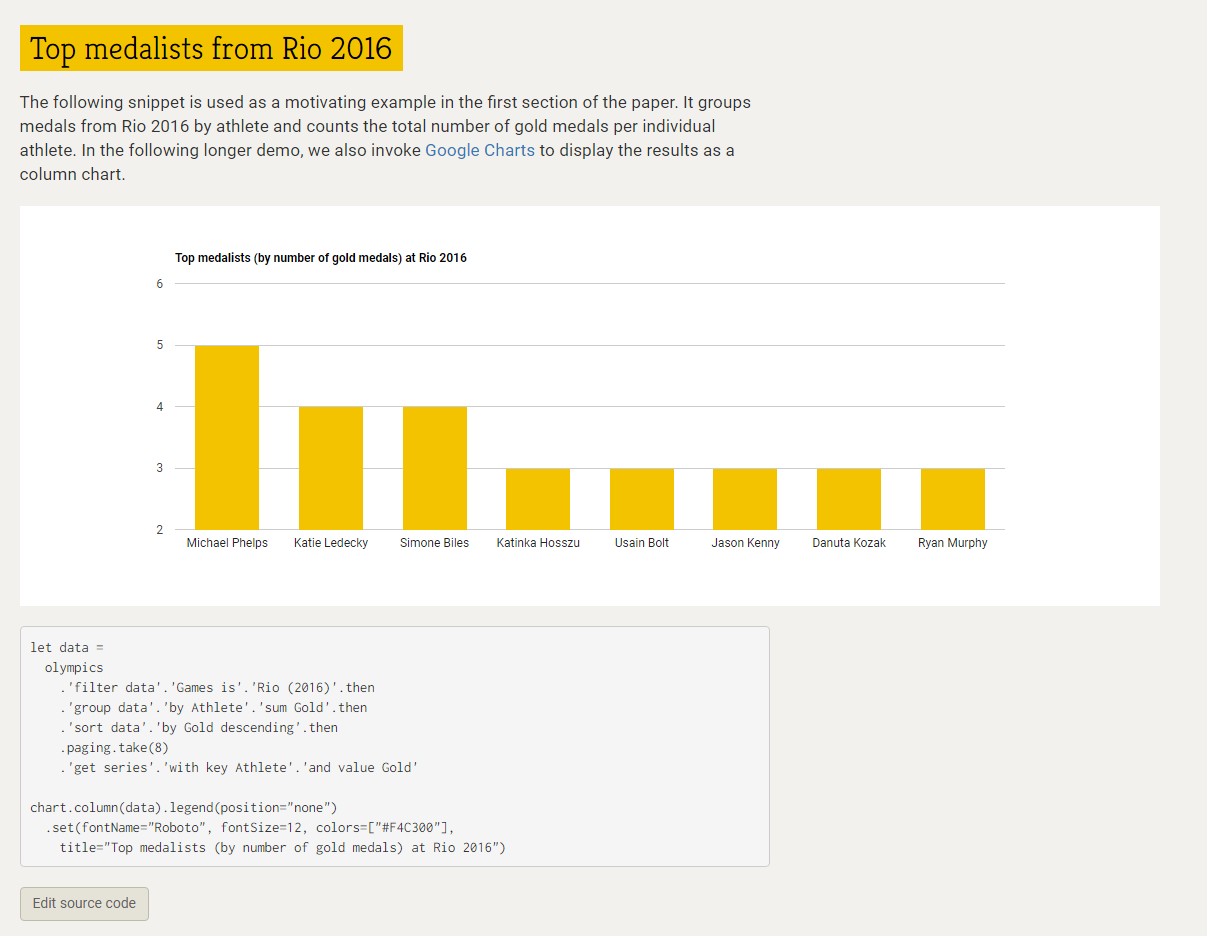
\includegraphics[scale=0.35,trim=0mm 0mm 0mm 0mm,clip]{images/af-preview.png}
\end{center}
\caption{Visualization showing top medalist from Rio 2016 with source code}
\label{fig:chart}
\end{figure}

\subsection*{Walkthrough 1: Obtain top medallists from London 2012}

In the first demo, we make a simple change to an existing source code to create a bar chart
showing top medallists from London 2012 rather than top medallists from Rio 2016.

\begin{enumerate}
\item Go to the first visualization ``Top medalists from Rio 2016'' and click the ``Edit source code''
  button to load the source code in the editor.
\item Locate the \texttt{Rio (2016)} member on the third line and delete it in the text editor.
  Additionally, delete the ``dot'' after \texttt{Games is}.
\item Type ``.'' immediately after the quoted \texttt{Games is} member. An auto-complete list
  should appear showing the available Olympic games together with their years.
  Choose \texttt{London (2012)} and make sure the identifier is separated from the following
  \texttt{then} member with another ``dot''.
\item Click ``Update page''. The visualization on the original demo page should change to show
  the new chart.
\end{enumerate}

\subsection*{Walkthrough 2: Obtain Mongolian gold medalists in code} 

This demo illustrates the experience of writing code using the pivot type provider from scratch.
We start with an empty code editor, start writing code and use auto-complete to create a simple
query.

\begin{enumerate}
\item Click on the ``Edit source code'' button for any of the examples and delete all source code
  in the editor, so that we can start from empty file.
  
\item Type \texttt{olympics.} and note that auto-complete offers different data transformations 
  as documented in the paper. Start by choosing \texttt{filter data}, followed by 
  \texttt{Team is} and \texttt{Mongolia}. Finally, complete the filtering by choosing \texttt{then}.
  Typing ``dot'' again offers the list of all available transformations.

\item Complete the query by typing ``dot'' and selecting items from auto-complete. When auto-complete
  is displayed, you can navigate using arrow keys and filter items by typing substrings of the
  member names. As you type, you can see the data calculated so far in the preview below the
  current line.

\begin{verbatim}
  olympics.'filter data'.'Team is'.Mongolia.then
    .'filter data'.'Medal is'.Gold.then.'get the data'
\end{verbatim}
  
\item Now that the data query is written, complete the sample by creating a table to show the results.
  Wrap the code in the following (note that the code written in previous step needs to be indented):

\begin{verbatim}
  let altan = (...)
  table.create(altan)   
\end{verbatim}

\item When you place the cursor inside the \texttt{table.create} call, you should see table as a
  preview. Click ``Update page'' and you should see the new table appear in the original demo page.
\end{enumerate}

\begin{figure}
\begin{center}
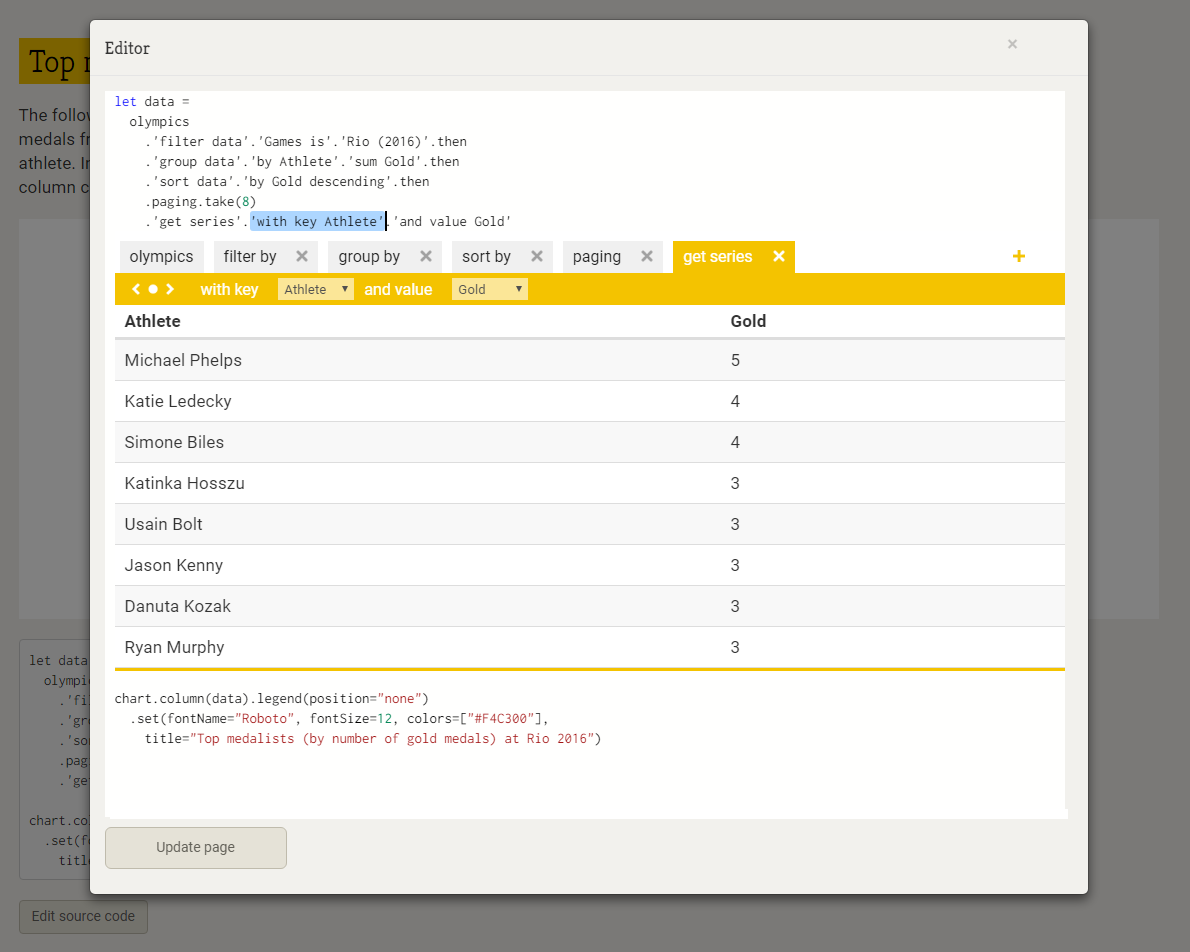
\includegraphics[scale=0.35,trim=0mm 0mm 0mm 0mm,clip]{images/af-editor.png}
\end{center}
\caption{Visualization showing top medalist from Rio 2016 with source code.}
\label{fig:code}
\end{figure}

\subsection*{Walkthrough 3: Count medals per discipline using the pivot user interface}

This demo introduces the user interface built on top of the pivot type provider as mentioned in the
case study presented in the paper. We will use the user interface to construct a simple query that
finds the number of medals awarded per discipline and finds the disciplines with the largest number
of medals. To do this, we make small edits to the code and complete the rest of the work using
a simple user interface.

\begin{enumerate}
\item Go to the ``All time medalists table'' demo and click ``Edit source code''.
\item In the displayed source code, click anywhere inside the query that performs the data aggregatoion
  so that the user interface displayed in Figure~\ref{fig:code} appears.
\item Remove all the operations except for \texttt{group by} by clicking on the ``x'' button on 
  the right. Start from the last one and remove \texttt{get the data}, \texttt{paging},
  \texttt{get the data} and \texttt{sort by}. Now, remove all the calculated aggregations 
  by clicking on ``x'' buttons in the yellow toolbar. 
\item Change the grouping key by selecting \texttt{by Discipline} in the drop down
  showing \texttt{by Athlete}. Next, add aggregation \texttt{count all} by clicking on the 
  ``+'' button in the yellow toolbar.
\item Add \texttt{sort by} transformation by clicking on the yellow ``+'' in the tab panel showing
  a list of operations. Then add sorting key \texttt{by count descending} by clicking on the ``+''
  in the yellow toolbar.    
\item Finally, add the \texttt{get the data} transformation to obtain the data. The final source
  code should look as follows:
\begin{verbatim}
  let data =
    olympics
      .'group data'.'by Discipline'.'count all'.then
      .'sort data'.'by count descending'.then
      .'get the data'
  table.create(data)  
\end{verbatim}
\item Finally, click ``Update page'' and review the newly produced table in the main page. You should
  see athletics at the top with 3856 medals and Jeu de Paume at the bottom with just 3 medals.
\end{enumerate}
\end{scope}

\begin{content}
The artifact package includes:
\begin{itemize}
\item a Docker image ({\tt thegamma-ecoop17.tar}), which contains the necessary client-side
  and server-side components for running the artifact
\item an F\# source code ({\tt thegamma-source.zip}) which contains the full source code for 
  the client-side and server-side components behind the artifact
\end{itemize}
To make evaluating of the user interface easier, we provide a Docker container that
can be used to host the system. The Docker container is based on the standard {\tt fsharp} 
image supplied by the F\# Software Foundation. 

The included source code provides complete source code
for the server-side components (running as F\# code on the server) and client-side components
(translated to JavaScript using the Fable compiler). When compiling code from scratch, several
packages are downloaded prior to the compilation from standard .NET and JavaScript package
repositories NuGet and npm.
\end{content} 

\begin{getting}

\subsection*{Running the artifact}
The presented artifact consists of a simple web server packaged as a Docker container. When 
started, the web server hosts the service that provides data to the web browser, as well as
a sample web page with a number of demos illustrating the language.

Running the artifact requires Docker (\url{https://www.docker.com}) and the Google Chrome 
browser (\url{http://www.google.co.uk/chrome}) and also download the provided
docker image \texttt{thegamma-ecoop17.tar}. To run the artifact, use the \texttt{docker load} command to 
unpack the image and \texttt{docker run} to start the web server:

\begin{verbatim}
    docker load --input thegamma-ecoop17.tar
    docker run -p 8889:80 thegamma-ecoop17
\end{verbatim}

\noindent
Alternatively, the \texttt{thegamma-ecoop17} Docker image is also hosted on the Docker repository
and can be downloaded and executed directly from the Docker repository:

\begin{verbatim}
    docker run -p 8889:80 tomasp/thegamma-ecoop17
\end{verbatim}

\noindent
The above commands specify the \texttt{-p 8889:80} parameter, which instructs Docker to map the
server hosted at port 80 inside the Docker container to a port 8889 of the host machine. Once
the Docker container starts, you will be able to access the sample web site by opening 
\url{http://localhost:8889} in the Google Chrome browser.

\subsection*{Latest version}  
The tool implemented as part of the submitted paper is also available as a JavaScript library
that is made available through the standard JavaScript package manager npm. The full
project soruce code is also hosted on GitHub. The following links can be used to obtain the latest
version:
\begin{itemize}
  \item \url{https://github.com/the-gamma/thegamma-script}
  \item \url{https://npmjs.com/package/thegamma-script}
\end{itemize}

\end{getting} 

\begin{platforms}
  The artifact is known to work on any platform running Docker version 17. It has been 
  specifically tested using Docker version 17.03.1-ce-win12 on the Windows operating system.
  5~GB of free space on disk and at least 2~GB of free space in RAM are sufficient for running
  the artifact.
\end{platforms}

\license{MIT ({\url https://opensource.org/licenses/MIT})}

% ARTIFACT: section specifying the md5 sum of the artifact master file
% uploaded to the Dagstuhl Research Online Publication Server, enabling 
% downloaders to check that the file is the expected version and suffered 
% no damage during download.
\mdsum{0e0e2873157bb6d69cbff5822523e41a}

% ARTIFACT: section specifying the size of the artifact master file uploaded
% to the Dagstuhl Research Online Publication Server
\artifactsize{335 MB}


% ARTIFACT: optional appendix
%\appendix

%\section{My Appendix}

% Add here any further material you would like to include. For instance, if the artifact is itself a PDF document, add it here.


% ARTIFACT: include here any additional references, if needed...

%% Either use bibtex (recommended), but commented out in this sample

%\bibliography{dummybib}

%% .. or use the thebibliography environment explicitely


\end{document}
